\chapter{Perancangan}
\label{chap:perancangan}

Pada bab ini akan dijelaskan mengenai perancangan Sistem Informasi Riwayat Mahasiswa yang akan dibuat. Mulai dari perancangan tampilan web yang digunakan, perancangan modul, dan perancangan diagram sekuens.


\section{Perancangan Tampilan Web Yang Digunakan}
\label{sec:perancanganantarmuka}

Perancangan tampilan web yang akan dibuat untuk mengimplementasikan Sistem Informasi Riwayat Mahasiswa terdapat lima buah perancangan yaitu pilih mahasiswa, info mahasiswa, edit mahasiswa, lihat histori dan entri baru.

\subsection{Tampilan Web Pilih Mahasiswa}
Perancangan tampilan web untuk pilih mahasiswa dapat dilihat pada Gambar~\ref{fig:pilihmahasiswa}.

\begin{figure}[H]
\centering
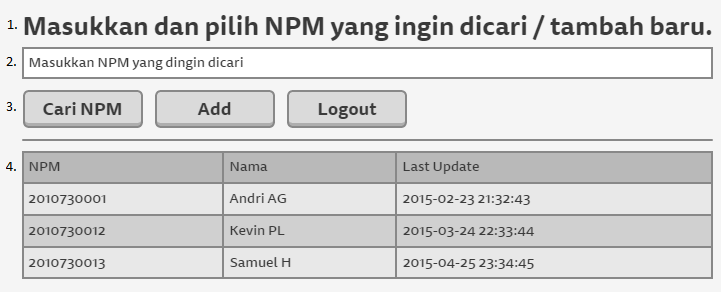
\includegraphics[scale=0.5]{Gambar/pilihmahasiswa.png}
\caption[Desain Antarmuka Pilih Mahasiswa]{Desain Antarmuka Pilih Mahasiswa}
\label{fig:pilihmahasiswa}
\end{figure}

Keterangan :
\begin{enumerate}[(1)]
\item
Bagian ini untuk memasukan input npm yang akan dicari oleh pengguna.
\item
Bagian ini merupakan tombol untuk melakukan aksi pencarian.
\item
Bagian ini merupakan tombol untuk melakukan aksi tambah data.
\item
Bagian ini merupakan tempat menampilkan data mahasiswa dalam bentuk tabel.
\end{enumerate}

\subsection{Tampilan Web Info Mahasiswa}
Perancangan tampilan web untuk info mahasiswa dapat dilihat pada Gambar~\ref{fig:infomahasiswa}.
\begin{figure}[H]
\centering
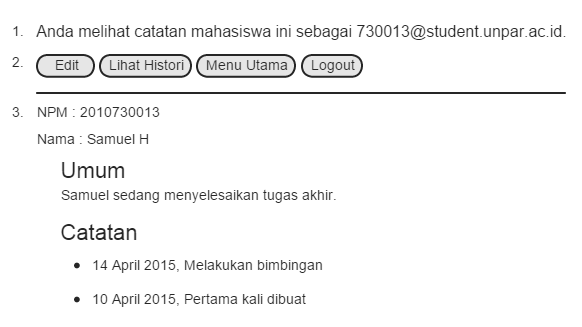
\includegraphics[scale=0.5]{Gambar/infomahasiswa.png}
\caption[Desain Antarmuka Info Mahasiswa]{Desain Antarmuka Info Mahasiswa}
\label{fig:infomahasiswa}
\end{figure}

Keterangan :
\begin{enumerate}[(1)]
\item
Bagian ini merupakan teks yang menampilkan keterangan dan juga pengguna yang sedang menggunakan Sistem Infomasi Riwayat Mahasiswa.
\item
Bagian ini merupakan tombol untuk melakukan aksi edit.
\item
Bagian ini merupakan tombol untuk melakukan aksi lihat histori.
\item
Bagian ini merupakan tempat menampilkan info mahasiswa yang berasal dari database.
\end{enumerate}

\subsection{Tampilan Web Edit Mahasiswa}
Perancangan tampilan web untuk edit mahasiswa dapat dilihat pada Gambar~\ref{fig:editmahasiswa}.
\begin{figure}[H]
\centering
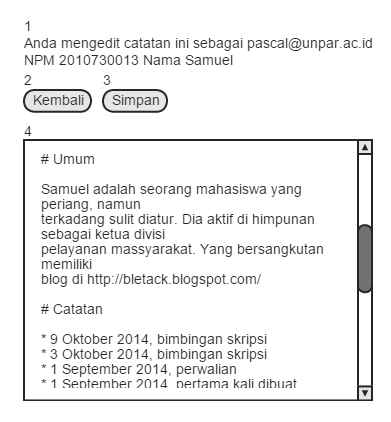
\includegraphics[scale=0.5]{Gambar/editmahasiswa.png}
\caption[Desain Antarmuka Edit Mahasiswa]{Desain Antarmuka Edit Mahasiswa}
\label{fig:editmahasiswa}
\end{figure}

Keterangan :
\begin{enumerate}[(1)]
\item
Bagian ini merupakan teks yang menampilkan keterangan dan juga pengguna yang sedang menggunakan Sistem Infomasi Riwayat Mahasiswa dan juga menampilkan NPM dan nama mahasiswa yang telah dipilih untuk diedit.
\item
Bagian ini merupakan tombol untuk melakukan aksi kembali ke info mahasiswa.
\item
Bagian ini merupakan tombol untuk melakukan aksi simpan untuk perubahan yang telah dilakukan.
\item
Bagian ini merupakan tempat menampilkan catatan mahasiswa yang berasal dari database dan dapat diedit (ditulis dengan foramt markdown).
\end{enumerate}

\subsection{Tampilan Web Lihat Histori}
Perancangan tampilan web untuk lihat histori dapat dilihat pada Gambar~\ref{fig:lihathistori}.
\begin{figure}[H]
\centering
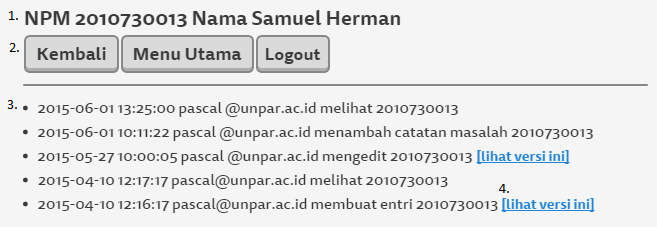
\includegraphics[scale=0.5]{Gambar/lihathistori.png}
\caption[Desain Antarmuka Lihat Histori]{Desain Antarmuka Lihat Histori}
\label{fig:lihathistori}
\end{figure}

Keterangan :
\begin{enumerate}[(1)]
\item
Bagian ini merupakan teks yang menampilkan keterangan NPM dan nama mahasiswa yang telah dipilih untuk dilihat historinya.
\item
Bagian ini merupakan daftar histori dari mahasiswa yang telah dipilih.
\end{enumerate}

\subsection{Tampilan Web Entri Baru}
Perancangan tampilan web untuk entri baru dapat dilihat pada Gambar~\ref{fig:entribaru}.
\begin{figure}[H]
\centering
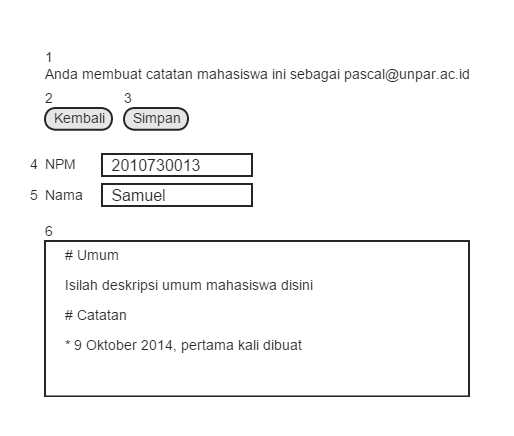
\includegraphics[scale=0.5]{Gambar/entribaru.png}
\caption[Desain Antarmuka Entri Baru]{Desain Antarmuka Pilih Entri Baru}
\label{fig:entribaru}
\end{figure}

Keterangan :
\begin{enumerate}[(1)]
\item
Bagian ini merupakan teks yang menampilkan keterangan dan juga pengguna yang sedang menggunakan Sistem Infomasi Riwayat Mahasiswa.
\item
Bagian ini merupakan tombol untuk melakukan aksi kembali ke pilih mahasiswa.
\item
Bagian ini merupakan tombol untuk melakukan aksi simpan untuk penambahan entri baru.
\item
Bagian ini merupakan area untuk memasukkan NPM mahasiswa yang akan ditambah.
\item
Bagian ini merupakan area untuk memasukkan nama mahasiswa yang akan ditambah.
\item
Bagian ini merupakan area  untuk memasukkan keterangan mahasiswa yang akan ditambah dengan format yang telah disediakan (ditulis dengan format markdown).
\end{enumerate}

\section{Perancangan Modul}
\label{sec:perancanganmodul}

Perancangan modul untuk Sistem Informasi Riwayat Mahasiswa yang akan dibuat dapat dilihat pada sub bab berikut.

\subsection{Modul Login}
Modul login yang dilakukan oleh user (dosen) dapat dilihat pada Tabel \ref{tab:modullogin}.

\begin{center}
\begin{table}
\caption[Tabel 4-1 Modul Login]{Modul Login}\\
\label{tab:modullogin}
\begin{center}
\begin{tabular}{ l p{10cm} }
\hline
Nama Modul & login.php\\
\hline
Input & username, password\\
\hline
Output & -\\
\hline
Tabel yang diakses & User\\
\hline
Deskripsi & User memasukkan username dan password kemudian sistem akan melakukan autentikasi menggunakan Google Oauth.\\
\hline
\end{tabular}
\end{center}
\end{table}
\end{center}

\subsection{Modul Pilih Mahasiswa}
Modul pilih mahasiswa yang dilakukan oleh user (dosen) dapat dilihat pada Tabel \ref{tab:modulpilihmahasiswa}.

\begin{center}
\begin{table}
\caption[Tabel 4-2 Modul Pilih Mahasiswa]{Modul Pilih Mahasiswa}\\
\label{tab:modulpilihmahasiswa}
\begin{center}
\begin{tabular}{ l p{10cm} }
\hline
Nama Modul & pilihmahasiswa.php\\
\hline
Input & npm\\
\hline
Output & Tabel mahasiswa\\
\hline
Tabel yang diakses & Mahasiswa\\
\hline
Deskripsi & User memasukkan npm yang ingin dicari, user juga dapat memilih langsung mahasiswa yang ingin dilihat infonya tanpa melakukan pencarian terlebih dahulu dan user juga dapat membaut entri baru.\\
\hline
\end{tabular}
\end{center}
\end{table}
\end{center}

\subsection{Modul Info Mahasiswa}
Modul info mahasiswa yang dilakukan oleh user (dosen) dapat dilihat pada Tabel \ref{tab:modulinfomahasiswa}.

\begin{center}
\begin{table}
\caption[Tabel 4-3 Modul Info Mahasiswa]{Modul Info Mahasiswa}\\
\label{tab:modulinfomahasiswa}
\begin{center}
\begin{tabular}{ l p{10cm} }
\hline
Nama Modul & infomahasiswa.php\\
\hline
Input & -\\
\hline
Output & Info mahasiswa\\
\hline
Tabel yang diakses & Mahasiswa\\
\hline
Deskripsi & User mendapatkan laporan barupa info mahasiswa yang telah dipilih sebelumnya pada modul pilih mahasiswa. User dapat merubah info mahasiswa yang ada dan dapat melihat histori setiap mahasiswa.\\
\hline
\end{tabular}
\end{center}
\end{table}
\end{center}

\subsection{Modul Edit Mahasiswa}
Modul edit mahasiswa yang dilakukan oleh user (dosen) dapat dilihat pada Tabel \ref{tab:moduleditmahasiswa}.

\begin{center}
\begin{table}
\caption[Tabel 4-4 Modul Edit Mahasiswa]{Modul Edit Mahasiswa}\\
\label{tab:moduleditmahasiswa}
\begin{center}
\begin{tabular}{ l p{10cm} }
\hline
Nama Modul & editmahasiswa.php\\
\hline
Input & teks dalam format markdown\\
\hline
Output & -\\
\hline
Tabel yang diakses & Mahasiswa\\
\hline
Deskripsi & User memasukkan atau merubah keterangan mahasiswa pada teks area yang telah disediakan menggunakan teks dengan format penulisan markdown lalu user menyimpan untuk menaruh perubahan yang dilakukan. User dapat kembali ke modul info mahasiswa tanpa melakukan perubahan.\\
\hline
\end{tabular}
\end{center}
\end{table}
\end{center}

\subsection{Modul Lihat Histori}
Modul lihat histori yang dilakukan oleh user (dosen) dapat dilihat pada Tabel \ref{tab:modullihathistori}.

\begin{center}
\begin{table}
\caption[Tabel 4-5 Modul Lihat Histori]{Modul Lihat Histori}\\
\label{tab:modullihathistori}
\begin{center}
\begin{tabular}{ l p{10cm} }
\hline
Nama Modul & lihathistori.php\\
\hline
Input & -\\
\hline
Output & Daftar histori mahasiswa\\
\hline
Tabel yang diakses & Mahasiswa\\
\hline
Deskripsi & User mendapatkan laporan berupa daftar hostori yang dimiliki setiap mahasiswa.\\
\hline
\end{tabular}
\end{center}
\end{table}
\end{center}

\subsection{Modul Entri Baru}
Modul entri baru yang dilakukan oleh user (dosen) dapat dilihat pada Tabel \ref{tab:modulentribaru}.

\begin{center}
\begin{table}
\caption[Tabel 4-6 Modul Entri Baru]{Modul Entri Baru}\\
\label{tab:modulentribaru}
\begin{center}
\begin{tabular}{ l p{10cm} }
\hline
Nama Modul & entribaru.php\\
\hline
Input & npm, nama, dan teks dalam format markdown\\
\hline
Output & -\\
\hline
Tabel yang diakses & Mahasiswa\\
\hline
Deskripsi & User memasukkan npm, nama, dan keterangan mahasiswa pada teks area yang telah disediakan menggunakan teks dengan format penulisan markdown lalu user menyimpan untuk membuat entri baru tersebut. User dapat kembali ke modul pilih mahasiswa tanpa melakukan perubahan.\\
\hline
\end{tabular}
\end{center}
\end{table}
\end{center}

\section{Diagram Sekuens}
\label{sec:diagramsekuens}

Pembuatan diagram sekuens mengacu pada Gambar~\ref{fig:usecase}. Diagram sekuens dapat dilihat pada Gambar \ref{fig:ds}.

\begin{figure}[H]
\centering
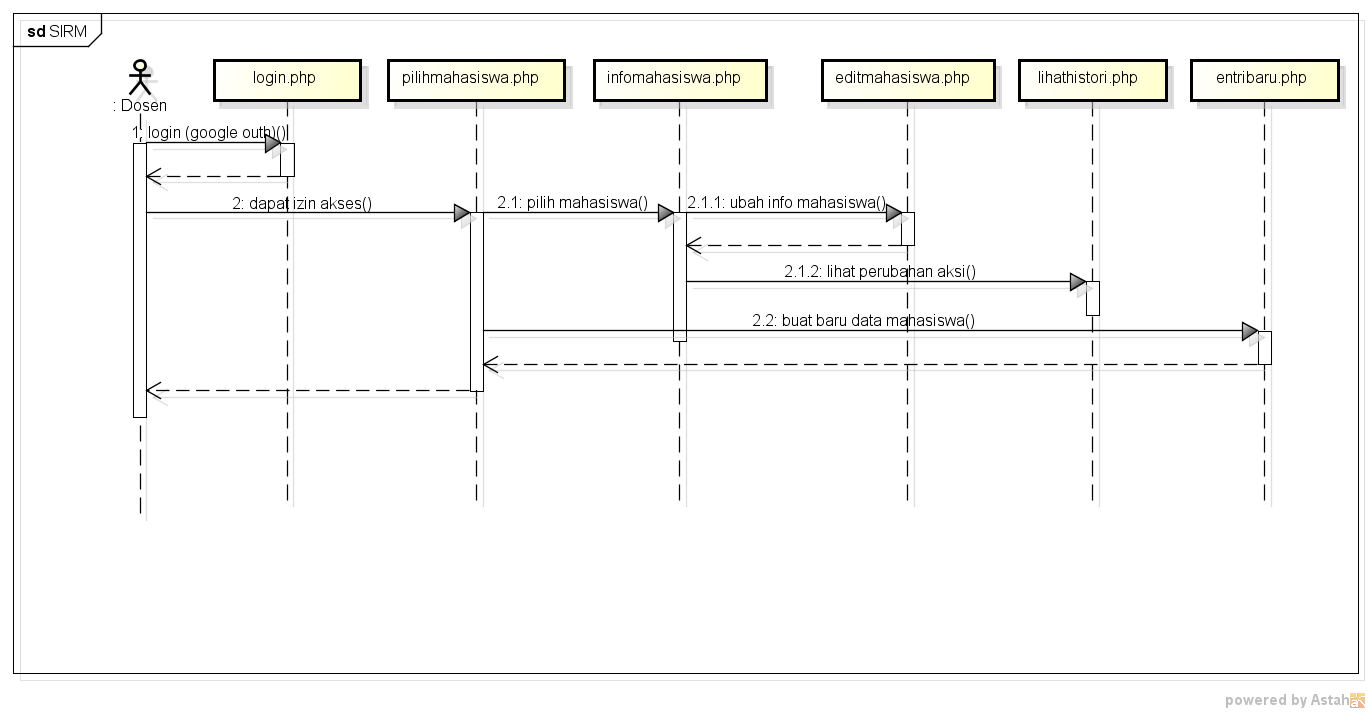
\includegraphics[angle=90,origin=c,scale=0.5]{Gambar/sekuens.png}
\caption[Diagram Sekuens]{Diagram Sekuens} 
\label{fig:ds}
\end{figure}